\chapter{Graphen}

\begin{figure}
    \centering
    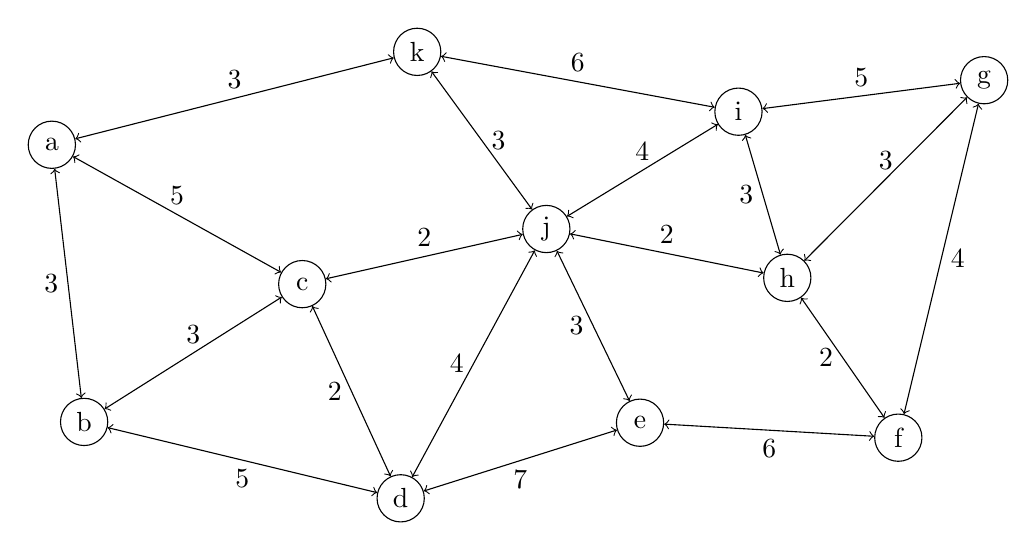
\begin{tikzpicture}
        % Nodes
        \node[circle, draw, minimum size=0.6cm, inner sep=0pt] at (1.60, -2.12)  (a)    {a};
        \node[circle, draw, minimum size=0.6cm, inner sep=0pt] at (2.01, -5.64)  (b)    {b};
        \node[circle, draw, minimum size=0.6cm, inner sep=0pt] at (4.78, -3.89)  (c)    {c};
        \node[circle, draw, minimum size=0.6cm, inner sep=0pt] at (6.03, -6.61)  (d)    {d};
        \node[circle, draw, minimum size=0.6cm, inner sep=0pt] at (9.07, -5.65)  (e)    {e};
        \node[circle, draw, minimum size=0.6cm, inner sep=0pt] at (12.35, -5.84)  (f)    {f};
        \node[circle, draw, minimum size=0.6cm, inner sep=0pt] at (13.44, -1.30)  (g)    {g};
        \node[circle, draw, minimum size=0.6cm, inner sep=0pt] at (10.94, -3.81)  (h)    {h};
        \node[circle, draw, minimum size=0.6cm, inner sep=0pt] at (10.32, -1.70)  (i)    {i};
        \node[circle, draw, minimum size=0.6cm, inner sep=0pt] at (7.88, -3.19)  (j)    {j};
        \node[circle, draw, minimum size=0.6cm, inner sep=0pt] at (6.24, -.94)  (k)    {k};


        \draw[<->]  (a) edge node[midway, left] {3} (b);
        \draw[<->]  (a) edge node[midway, above] {5} (c);
        \draw[<->]  (a) edge node[midway, above] {3}  (k);

        \draw[<->]  (b) edge node[midway, above] {3} (c);
        \draw[<->]  (b) edge node[midway, below] {5} (d);

        \draw[<->]  (c) edge node[midway, left] {2} (d);
        \draw[<->]  (c) edge node[midway, above] {2} (j);

        \draw[<->]  (d) edge node[midway, left] {4} (j);
        \draw[<->]  (d) edge node[midway, below] {7} (e);

        \draw[<->]  (e) edge node[midway, left] {3} (j);
        \draw[<->]  (e) edge node[midway, below] {6} (f);

        \draw[<->]  (f) edge node[midway, right] {4} (g);
        \draw[<->]  (f) edge node[midway, left] {2} (h);

        \draw[<->]  (g) edge node[midway, above] {3} (h);
        \draw[<->]  (g) edge node[midway, above] {5} (i);

        \draw[<->]  (h) edge node[midway, left] {3} (i);

        \draw[<->]  (i) edge node[midway, above] {4} (j);
        \draw[<->]  (i) edge node[midway, above] {6} (k);

        \draw[<->]  (j) edge node[midway, right] {3} (k);
        \draw[<->]  (j) edge node[midway, above] {2} (h);
    \end{tikzpicture}
    \caption{Beispielgraph}
\end{figure}

\todo{Graphen auf Kinderniveau erklären und schöne Bilder von Graphen zeigen}.

\section{Definitionen}
Damit in den nachfolgenden Kapiteln sinnvoll argumentiert werden kann, ist es notwendig, einige Begriffe zu definieren.

\begin{definition}[Graph]
    Sofern nicht anders angegeben, wird ein endlicher, gerichteter Graph mit Kantengewichten, ohne Mehrfachkanten und Schleifen, einfach als Graph bezeichnet.

    Als Schreibweise wird $G = (V, E)$ verwendet, wobei $V$ die Knotenmenge und $E$ die Kantenmenge ist. Eine Kante ist ein Tupel $(t, h, w)$. $t \in V$ wird als \emph{Fuß}, $h \in V$ als \emph{Kopf} und $w \in \mathbb{R}$ als \emph{Gewicht} bezeichnet. Gelegentlich wird auch nur $(t, h)$ geschrieben, um auszudrücken, dass zwei Knoten verbunden sind. Da ein Graph keine Mehrfachkanten zulässt, definiert diese Schreibweise auch eindeutig das Kantengewicht.

    Wird $G$ als ungerichtet bezeichnet, dann gilt $(t, h) \in E \Leftrightarrow (h, t) \in E$.
\end{definition}

In einem Graphen gibt es oft das Interesse, von einem Knoten zu einem anderen zu gelangen.
Diese Verbindungen zwischen Knoten werden durch sogenannte Wege dargestellt.

\begin{definition}[Weg]
    Ein Weg auf einem Graph $G = (V, E)$ ist eine Folge von Knoten $v_1, \dotsc, v_n$, für die gilt, dass benachbarte Knoten im Weg eine Kante in $E$ bilden.

    \todo{Wie nenne ich die Hoplänge?}

    Die Summe der Kantengewichte aller Kanten $(v_i, v_{i + 1})$ wird \emph{Länge} des Weges genannt. Der Knoten $v_1$ wird Startknoten, $v_n$ Zielknoten genannt.
\end{definition}

Zwischen zwei Knoten kann es mehrere unterschiedliche Wege geben.
Diese Wege können auch unterschiedliche Länge haben.

\begin{definition}[Kürzester Weg]
    Ein Weg $v_1, \dotsc, v_n$ ist \emph{ein kürzester Weg}, wenn die Länge des Weges unter allen Wegen von $v_1$ nach $v_n$ minimal ist. Die Länge des kürzesten Weges wird als \emph{Abstand} von $v_1$ und $v_n$ bezeichnet. Die Definition des Graphen lässt es zu, dass es mehrere kürzeste Wege zwischen zwei Knoten gibt.

    Sei $P \subset V \times V$ die Menge der Knoten, zwischen denen ein Weg existiert. Dann sind definiert:
    \begin{enumerate}
        \item
              ${spd} \colon P \to \mathbb{R}$ weist einem Knotenpaar den Abstand zu.

        \item
              ${sp} \colon P \to V \times V \times \dots \times V$ weist einem Knotenpaar einen kürzesten Weg zu.
    \end{enumerate}
\end{definition}

\begin{definition}[Umkehrgraph]
    Sei $G = (V, E)$ ein Graph. Dann ist $G^T = (V, E^T)$ mit $(t, h, w) \in E \Leftrightarrow (h, t, w) \in E^T$ der \emph{Umkehrgraph} von $G$.
\end{definition}

Zusätlich zum finden eines Weges zwischen zwei Knoten ist es häufig notwendig den kürzesten Weg von einem Knoten zu allen anderen Knoten zu finden.
Auch die Umkehrung dieses Problem ist interesannt, also die kürzesten Wege von allen Knoten zu einem zu bestimmen.
Diese Probleme sind äuivalent, da das Finden alle kürzesten Wege zu einem Knoten auf einem Graph $G$ dem Finden aller kürzester Wege auf dem Umkehrgraph $G^T$ entspricht.

\section{Nicht-Straßen Graphen}



Kürzeste Pfad Queries mit dem klassischen Dijksta Algorithmus sind auf den visibility Graphen deutlich teuerer als auf den triangulierten Graphen.


Fokus dieser Arbeit erklären.

Unterschiede zwischen Straßengraphen und NIcht-Straßengraphen erklären.
TODO Straßengrqaphen sind hierarchisch, aber was heist das genau.
TODO kann ich mit einer Metrik binär unterteilen ob ein GraPh hierarisch ist?

Die graph erklären, die ich mir speziell anschaue.
Trianguliereung erklären TODO Daniel?

Graphen zeichen, metriken zeichen.
Degree Plot
Hitting Set Plot?
Sonstige Metriken? TODO Funke


shasum graphen
6c00147bf26a2c37e50db857f4ce4ab565a236dd  aegaeis-ref-graph.fmi
acdf08813a59534840c605984e9c37875f77f32a  aegaeis-ref-visibility.fmi
b22697934378f6f8af7fb7bf3ae2812d7b0029ec  medi-ref-graph.fmi
77760c910a13f9dc056f4ef3f3f532b00286c52f  medi-ref-visibility.fmi
b9727caf46fd3407ce0b5e2b08b941dfb15f95f6  pata-ref-graph.fmi
89356e6e6411b8340375c3aa0fc949fb4e58ff44  pata-ref-visibility.fmi


\section{Dijkstra}

\todo{Dijkstra Algorithmus erklären und Dijkstra Paper zitieren}

Ziel ist nicht Dijktra selbst, sondern folgende Metriken erklären.

\todo{Dijkstra Rank}
\todo{Queue Pops}
\todo{Max Queue len}

\section{Datenstrukturen}

Verschieden Graph Strukturen

Grundlegende Idee:
Ein Interface Graph welches nur ausgehende Kanten kennt.
get edge distance, set edge distance

Dieses habe ich für verschiedene Graphen implementiert.
Wichtigste:
VecVec: Ein Vec. Jeder Vertex hat hat einen Eintrag vom Typ Vec in dem die kanten sortiert nach Head sind.
VecHashMap: Ein Vec. Jeder Vertex hat einen Eintrag vom Typ HashMap (Head, Distance).
Vec: Zwei Vec. Einer für (Head, Distance), zweiter für startindex, stopindex für Vec.
TODO Indexmap?

Häufig eine Abwägung wie schnell gequeriet werden kann vs wie schnell bearbeitet werden kann.


für reverse dijkstra uä muss aber auch Vorgänger bekannt sein.
Idee: Reversible Graph aus einem Vorwärtsgrapg und Rückwärtgraph
Beide sind aber grundätzlich gleiche Struktur. Daher ist Vorwärts und Rückwärtssuche gleiche Funktion.


Gleiches gilt für Contracted Graph. Zwei Graphen Upward Graph und Downward Graph. Downward Graph ist aber \"umgedreht\" zur Definition aus dem Paper, es wird also beides mal eine Vorwärtssuche gemacht.


\section{Archivierung}

Zum Speichern von Graphen wird ein Text Based Format benutzt.


Beliebig viele Kommentar lines
leere line
num Vertices
num Edges
Vertices
Edges

Suche
Für Dijkstra verscheidene Datenstrukturen getestet.
Data (predecessor, distance)
Queue (min heap)
is\_expanded

jeweils ein Interface.

TODO. Testen verschiedener Kombinationen.
TODO. Wann ist reuse of allocation sinvoll?
TODO Decrease key


